\section{Drift Chamber Electronics}

In this section we describe the drift chamber electronics:
the on-chamber signal distribution and amplification boards, which
we named ``Signal Translator Boards'', (STBs),
the on-chamber high voltage translator boards (HVTBs), and the
off-chamber drift chamber readout boards (DCRBs).

On one endplate of each chamber is a set of HVTBs that distribute RC-filtered high voltage
to the wires.  Because there are three types of wire, (sense, field, and guard), we supply
three different voltages to each HVTB board.  

On the other side of the chamber are the STBs that support an individual Single Inline Package
(SIP) transimpedance preamplifier that is capacitively coupled to each sense wire since the
sense wires are at high voltage.  This preamplifier takes the
small current pulse (as small as a few $\mu$A) and translates it into a voltage 
pulse with a transimpedance of 2~mV/$\mu$A.  The signals (typically
10s to 100s of mV and 10s to 100s of ns duration) are
transmitted down (17-pair) twisted-pair cables to our downstream DCRBs that further amplify and
discriminate the voltage pulses and then convert the leading edge
to a digital time signal.

The drift chamber signal amplification and readout system thus consists of the following:
\begin{itemize}
\item  chamber-mounted printed circuit boards with an amplifier for each signal wire; 
these are the STBs (one type for each superlayer);
\item  chamber-mounted printed circuit boards that distribute high voltage
to all of the wires; these are the HVTBs (one type for each superlayer);
\item a single 17-pair twisted-pair readout cable for each group of 16
SIPs;
\item a 96-channel DCRB for each group of 6 cables (96 signal wires).
\end{itemize}

Table ~\ref{electronic-components} gives a channel count for our chamber-mounted electronic components.

%%%%%%%%%%%%%%%%%%%%%%%%%%%%%%%%%%%%%%%%%%%%%%%%%%%%%%%%%%%%%%%
\begin{table}[htbp]
\begin{center}
\begin{tabular} {||c|c||} \hline \hline
{\bf Component}           & {\bf Number} \\ \hline
STB boards (6 types)      & 252 total \\ \hline
HVTB boards (6 types)     & 252 total \\ \hline
low-voltage cables        & 252 total  \\ \hline
high-voltage cables       & 252 total  \\ \hline
signal cables (17-pair)   & 1512 \\ \hline
total signals             & 24192 \\ \hline \hline
\end{tabular}
\caption{\small{Electronic channel counts for the readout, high voltage,
and low voltage systems for the drift chambers.}}
\label{electronic-components}
\end{center}
\end{table}
%%%%%%%%%%%%%%%%%%%%%%%%%%%%%%%%%%%%%%%%%%%%%%%%%%%%%%%%%%%%%%%

\subsection{STB and HVTB: Installation and Use}
\label{stb-hvtb-installation}

The high voltage side of each chamber was tiled with 14  multi-layered printed circuit 
boards, (HVTB). The HVTBs were designed to distribute three
separate voltages to the sense, field, and guard wires, respectively.  See
Section~\ref{determine-operating-parameters} for a 
description of how we determined the operating values of the high voltage.

The board layout is shown in Fig.~\ref{hvtb-layout}.
Each high voltage cable is connected to a low-pass filter (with R=1M$\Omega$ and C=1pF) to 
eliminate any high frequency noise from the supplies.
The filtered power is then passed to the 4-layer printed circuit
portion for distribution to the sense, field and guard wires.
To limit any potential high voltage breakdown, there is a 1 M$\Omega$
resistor for each sense wire.
%%%%%%%%%%%%%%%%%%%%%%%%%%%%%%%%%%%%%%%%%%%%%%%%%%%%%%%%%%%%%%%%
\begin{figure}[htbp]
\vspace{8cm}
\begin{picture}(50,50)
\put(50,20)
{\hbox{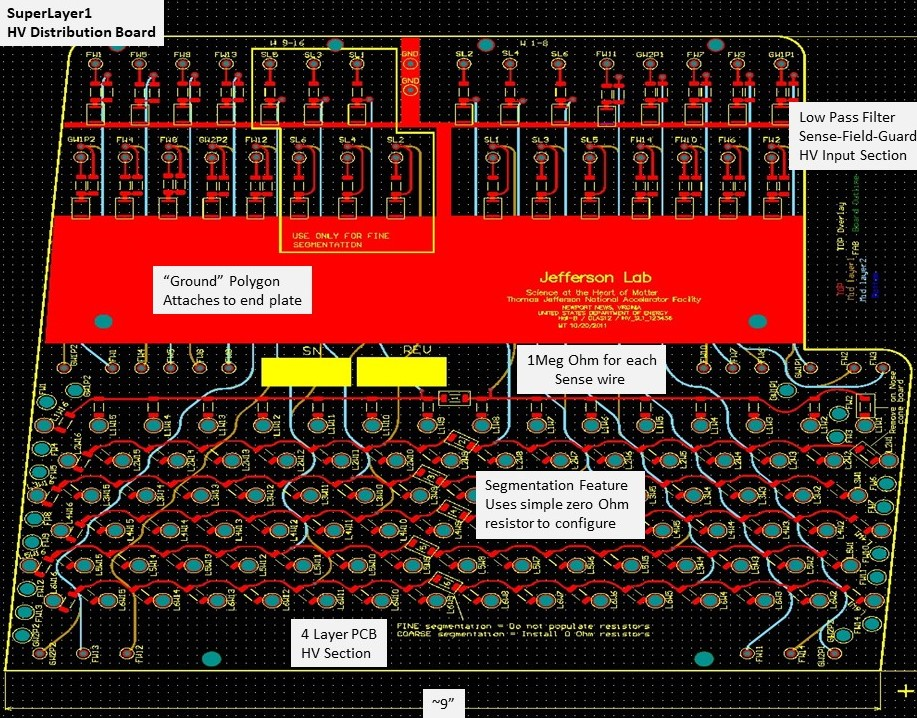
\includegraphics[width=0.7\textwidth,natwidth=610,natheight=642]{img/hvtb-layout.jpg}}}
\end{picture}
\caption{\small{Board layout drawing for the high-voltage translator boards.}}
\label{hvtb-layout}
\end{figure}
%%%%%%%%%%%%%%%%%%%%%%%%%%%%%%%%%%%%%%%%%%%%%%%%%%%%%%%%%%%%%%%%

The signal side of each chamber was tiled with 14 multi-layered printed circuit 
boards, (STB).  These boards were built in a 96-channel format that
requires seven circuit boards for each superlayer (672 signals). The boards capacitively
decoupled high-voltage from the signals, and then routed 
the signals to the SIP transimpedance preamplifiers 
mounted on the boards.  The amplified differential signals are then sent 
via 20-m long twisted-pair lines to the main CLAS12 readout electronics.

Fig.~\ref{stb-layout} shows the layout of an STB board,
including the trace routings from the capacitively-coupled
wire signal to the SIP and the
placement of the SIPs into groups of 16 with the SIP outputs being
routed to the 16-pin signal connectors.  Also shown are the low-voltage
power traces with individual negative voltage regulators for each
group of 16 preamplifiers.  The negative voltage regulators were connected
in isolation mode to provide +5VDC regulated voltage to the group
of 16 preamplifiers.  The board shown is from a R1 chamber, which
had the tightest wire and trace density.

%%%%%%%%%%%%%%%%%%%%%%%%%%%%%%%%%%%%%%%%%%%%%%%%%%%%%%%%%%%%%%%%
\begin{figure}[htbp]
\vspace{12cm}
\begin{picture}(50,50)
\put(20,5)
{\hbox{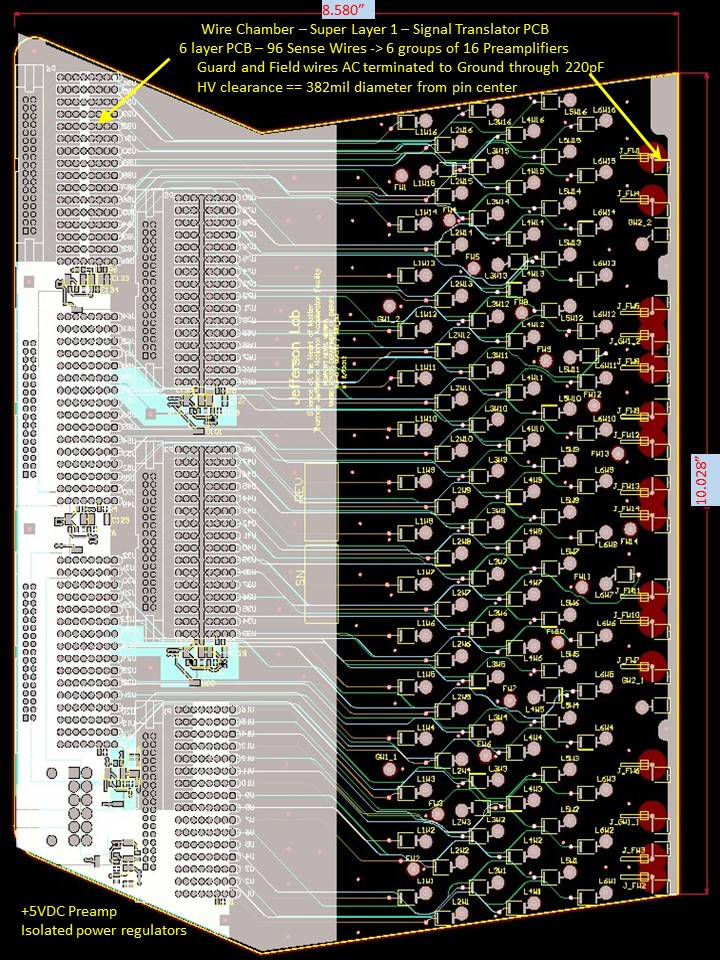
\includegraphics[width=0.35\textwidth,natwidth=610,natheight=642]{img/stb-layout.jpg}}}
\end{picture}
\caption{\small{Trace routing shown on one of the Region~1 STBs.}}
\label{stb-layout}
\end{figure}
%%%%%%%%%%%%%%%%%%%%%%%%%%%%%%%%%%%%%%%%%%%%%%%%%%%%%%%%%%%%%%%%

The connections between the sense-wire crimp pins and the plated-through holes 
of the STB boards were made using short conductive-elastomer tubes. This material 
consists of silver-plated and/or nickel-plated glass spheres embedded in a 
silicon-rubber matrix. These tubes pass through the plated-through hole and 
over the end of the crimp pins, making the electrical contact between the 
wire and the circuit board.  A small plastic cap inserted into the end of the 
tube ensures good contact with the circuit board.  This approach has the 
advantages of reducing the space needed for connections, preventing crimp pins 
from being pulled from the feedthroughs when disconnecting the boards from the 
wires, and reducing the cost compared to metal connectors.  This detail is 
shown in Fig.~\ref{wire-to-amplifier}.

%%%%%%%%%%%%%%%%%%%%%%%%%%%%%%%%%%%%%%%%%%%%%%%%%%%%%%%%%%%%%%%
\begin{figure}[htbp]
\vspace{8.5cm}
\begin{picture}(50,50)
\put(30,5)
{\hbox{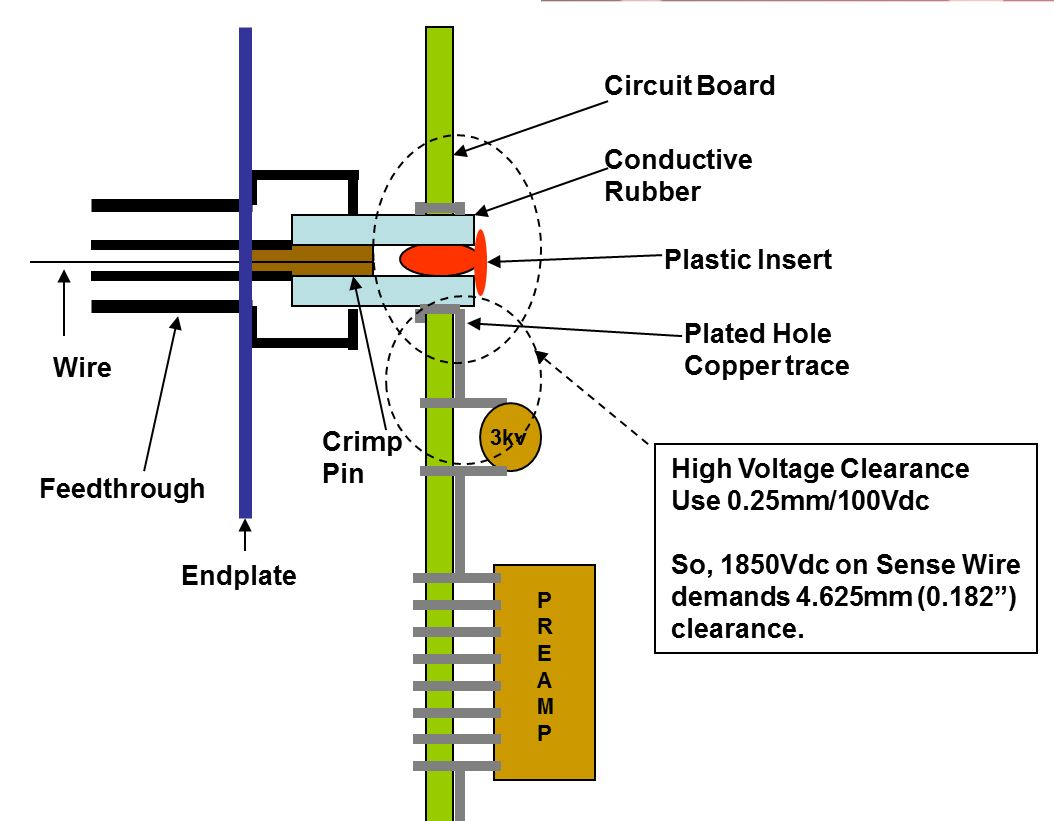
\includegraphics[width=0.7\textwidth,natwidth=610,natheight=642]{img/wire-to-amplifier.jpg}}}
\end{picture}
\caption{\small{ An assembly drawing showing how the crimp pin was inserted
into the feedthrough and how the conductive elastomer tube fits over the 
crimp pin and inside the plated-through hole on the printed circuit board to 
make the electrical connection. Also shown is the signal path from the wire's
crimp pin to the preamplifier.}}
\label{wire-to-amplifier}
\end{figure}
%%%%%%%%%%%%%%%%%%%%%%%%%%%%%%%%%%%%%%%%%%%%%%%%%%%%%%%%%%%%%%%%



\subsubsection{Single Inline Package Preamplifiers}

The heart of the STB board is an individually packaged
single in-line package (SIP) preamplifer that was modified
from the design of the previous CLAS detectors and 
included an epoxy resin encapsulation.  
The encapsulation of the components prevents 
component corrosion in a somewhat humid environment (relative
humidities as high as 60\%).
These ``CP01'' preamplifiers provide the gain, dynamic range, rise time, low 
noise, and low power needed for the performance requirements.  The CP01 is
a transimpedance amplifier with a gain of 2 mV/$\mu$A and a rise-time
of less than 10 ns.  Each SIP operates at 5 V and draws about 13 mA.   
Fig.~\ref{CP01-description} shows the design and specifications of the
CP01 preamplifier.  See Ref.~\cite{fjb92} for the original design of
this SIP preamplifier.

%%%%%%%%%%%%%%%%%%%%%%%%%%%%%%%%%%%%%%%%%%%%%%%%%%%%%%%%%%%%%%%%%
\begin{figure}[htbp]
\vspace{8cm}
\begin{picture}(50,50)
\put(40,5)
{\hbox{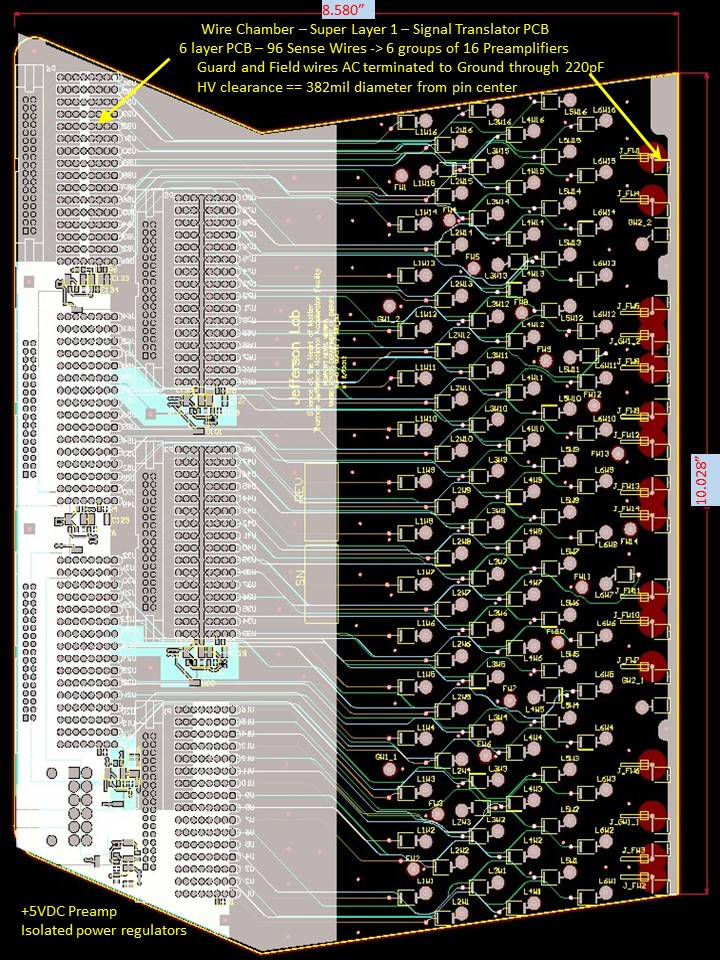
\includegraphics[width=0.7\textwidth,natwidth=610,natheight=64]{img/CP01-description.jpg}}}
\end{picture}
\caption{\small{The CP01 preamplifier design and specifications.}}
\label{CP01-description}
\end{figure}
%%%%%%%%%%%%%%%%%%%%%%%%%%%%%%%%%%%%%%%%%%%%%%%%%%%%%%%%%%%%%%%%%

Each group of 16 preamplifier output signals was routed to a 17-pair connector.
Sixteen of the pairs are used as differential signal paths that are routed from the STBs to the 
DCRBs over individual cables consisting of 16 twisted pairs. We chose
twisted-pair readout because of its immunity to electronic noise.
The cables are round-jacketed with a 
0.025-in pitch so that the overall cable dimension is smaller than the 
standard 17-pair cable.  

\subsection{Off-Chamber Amplification, Time Digitization, and Readout}

Our on-chamber preamplifiers send signals to the DCRBs, which provide another level of amplification, 
signal discrimination, adjustable threshold setting, time digitization, and readout. 



\subsubsection{Drift Chamber Readout Boards}

The DCRB is a 96-channel board that is a combination post-amplifier,
discriminator and time-to-digital converter (TDC); it also has a trigger
output path to provide track segment information for an online tracking trigger.
Fourteen such boards are housed in
a proprietary 9U, 160 mm depth, VXS form factor crate.
The whole system consisted of 18 such crates, one for each drift chamber.
See Ref.~\cite{daq-nim} for more details.

These DCRBs are based on FPGA technology, and in addition to
their primary function of amplification, discrimination, digitization,
and readout, they are used in a simple ``cluster-finding'' algorithm
to find track segment candidates with a latency of only hundreds
of nanoseconds.  For a more complete description of this please
see our companion article on the trigger, Ref.~\cite{trigger-nim}.

To perform its time digitization task, the DCRB utilizes on-board synchronization to
return the signal time relative to an input time signal from  a Trigger Distribution
Crate. Its design and architecture
allows it to achieve the following performance metrics:
\begin{itemize}
\item DCRB Performance Metrics
\begin{itemize}
\item Amplification: variable gain from X10 to X30 eliminates saturation
\item Time Digitization: accuracy better than 1 ns; exceeds DC specifications
\item Whole Crate Time Synchronization: through backplane; eliminates cables
\item Event Buffer Size: 500,000 signals
\item VME Transfer Rate: 200~MB/s
\item Maximum Trigger Rate: greater than 1~MHz
\item Dead-time: 32~ns
\item Scaler: 1 32 bit scaler per channel
\item Track Segment Finding: employs segment-hit dictionary in 32~ns bins
\item Track Segment Reporting: reports found segments to the next-level Track Finder
\end{itemize}
\end{itemize}

In addition to its primary functions of time digitization of DC signals and online
track-finding, the internal scaler functions allow the DCRB to be used in 
a stand-alone manner to efficiently monitor chamber operation during commissioning
and testing.

\subsection{Grounding Scheme}


We used a single point grounding scheme, where the single point ``ground'' or zero reference was 
the CAEN high-voltage power supply crates.  Two return (ground) wires were used on every 
high-voltage module output, and these ground wires were carried through to the HVTB's which were 
grounded to the drift chamber end plates.  The drift chambers themselves were insulated from the 
torus magnet through use of an insulating portion of the link mounting system. The off-chamber DCRBs 
were likewise not grounded to the chambers through the use of non-grounded twisted-pair 
signal cables. The low-voltage power supplies were floating, supplying a plus and minus line to the 
+5VDC regulators on the STB's. 
